\documentclass[10pt]{article}
\usepackage[
  paperwidth=595.22pt,
  paperheight=842pt,
  margin=0pt
]{geometry}
\usepackage{fontspec}
\usepackage{xeCJK}
\usepackage{graphicx}
\usepackage{xcolor}
\usepackage{tikz}
\pagestyle{empty}

\setmainfont{Arial}
\setsansfont{Arial}
\setCJKmainfont{SimSun}
\setCJKsansfont{SimSun}

\definecolor{textblack}{RGB}{30,30,30}
\definecolor{rulegray}{RGB}{145,145,145}
\definecolor{labelgray}{RGB}{50,50,50}

\newcommand{\putat}[3]{%
  \begin{tikzpicture}[remember picture,overlay]
    \node[anchor=north west,inner sep=0pt] at
      ([xshift=#1,yshift=-#2]current page.north west) {#3};
  \end{tikzpicture}%
}

\newcommand{\textboxat}[5]{%
  \begin{tikzpicture}[remember picture,overlay]
    \node[
      anchor=north west,
      inner sep=0pt,
      text width=#3,
      align=#4,
      text=textblack
    ] at ([xshift=#1,yshift=-#2]current page.north west) {#5};
  \end{tikzpicture}%
}

\begin{document}
\mbox{}

% Header and footer stay unchanged from the source page.
\textboxat{72pt}{38.4pt}{55pt}{left}{%
  {\fontsize{11.2}{13}\selectfont 1P5}%
}
\putat{158pt}{39.0pt}{%
  \resizebox{280pt}{!}{%
    {\fontsize{10.4}{12}\selectfont
    P5 Thermodynamics Lab: Background \& Prep}%
  }%
}
\textboxat{408pt}{38.4pt}{134pt}{right}{%
  {\fontsize{11.2}{13}\selectfont Page 18 of 52}%
}
\textboxat{72pt}{792.4pt}{280pt}{left}{%
  {\fontsize{10.2}{12}\selectfont P5 Thermo PrepWork 2526.docx}%
}
\textboxat{402pt}{792.4pt}{140pt}{right}{%
  {\fontsize{9.4}{11.2}\selectfont Jan-2026}%
}

% Original figure panels, cropped from the source PDF and preserved as images.
\putat{132pt}{63pt}{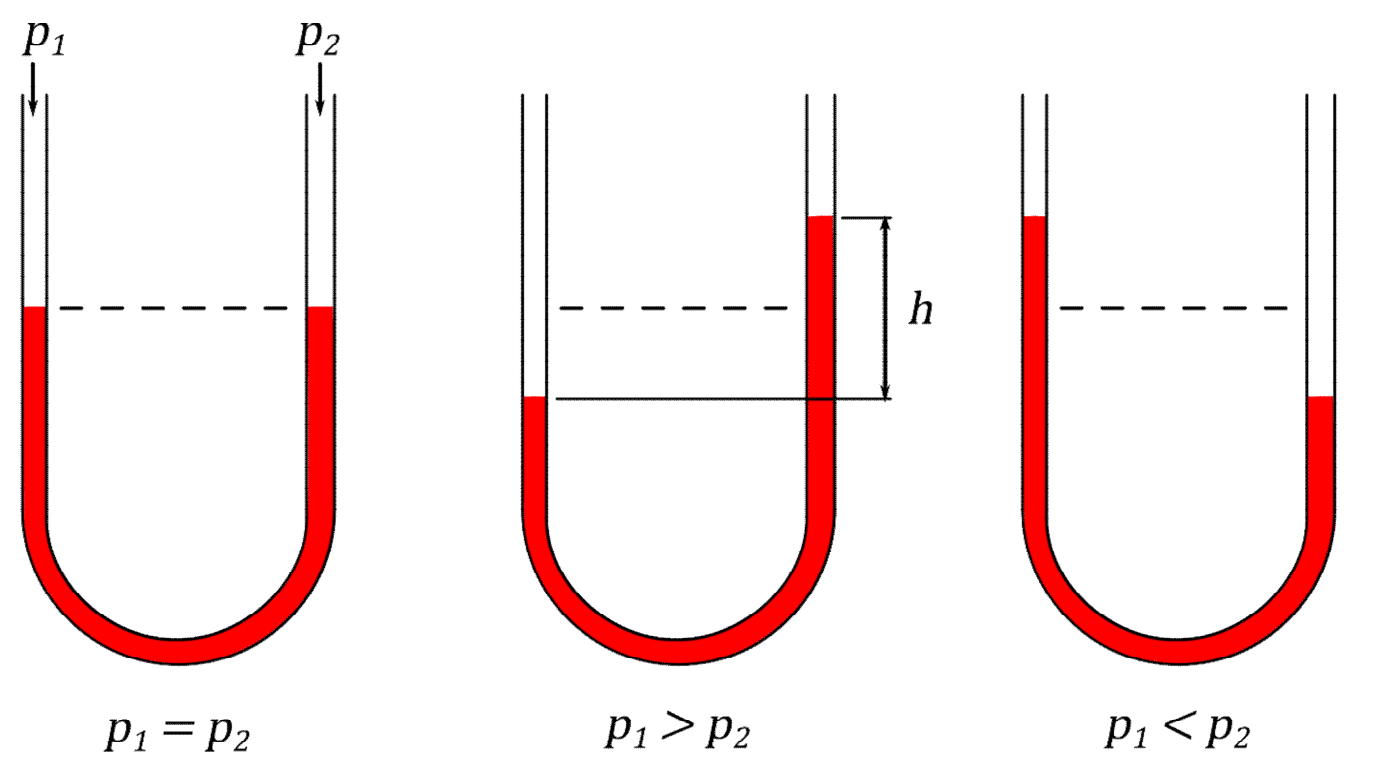
\includegraphics[width=346pt]{p18_panel_a_utube.png}}
\putat{132pt}{283pt}{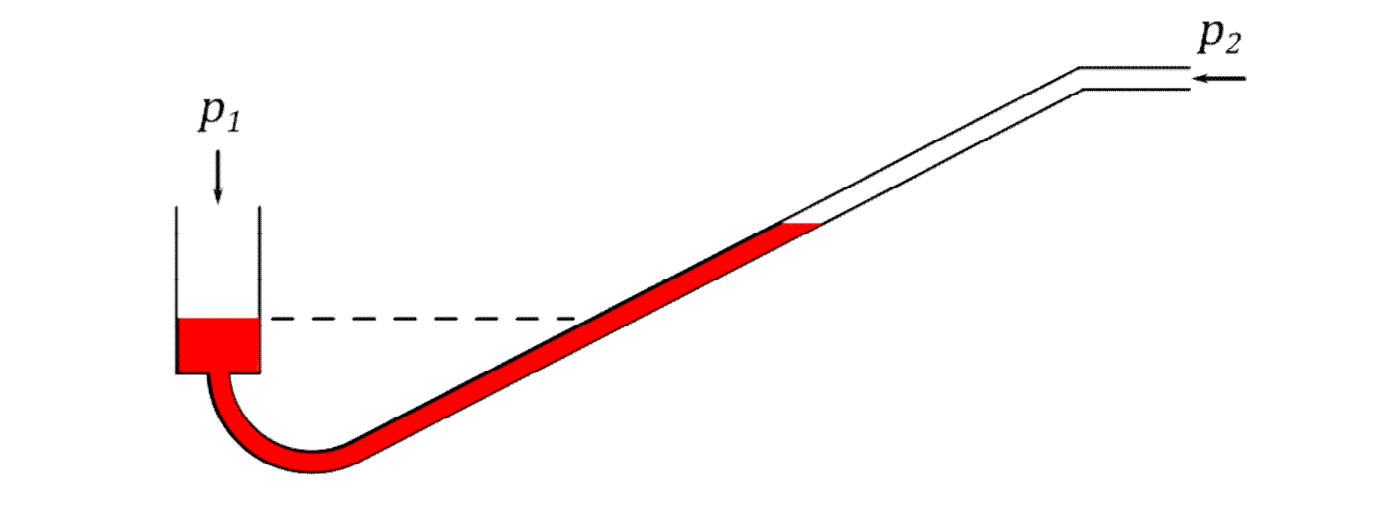
\includegraphics[width=346pt]{p18_panel_b_inclined.png}}
\putat{132pt}{436pt}{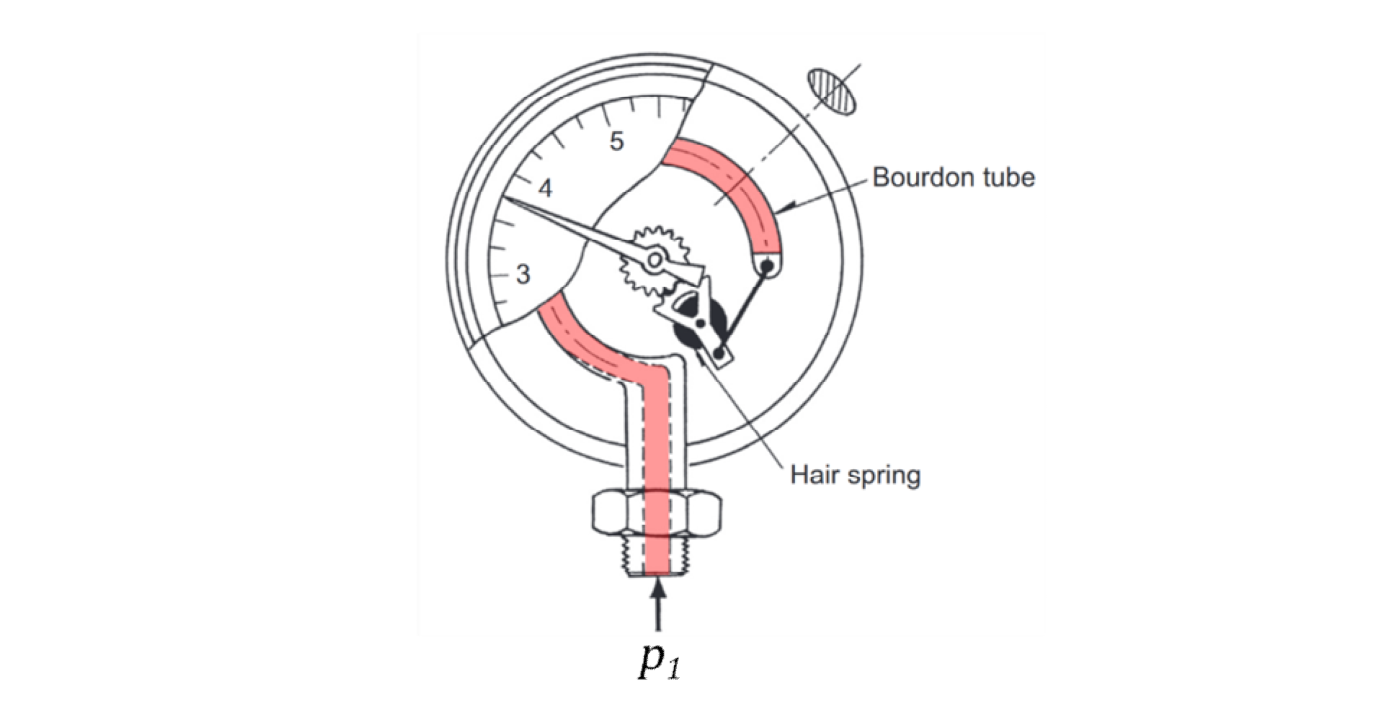
\includegraphics[width=346pt]{p18_panel_c_bourdon.png}}

% Bilingual captions replacing the source captions.
\textboxat{132.4pt}{263.3pt}{260pt}{left}{%
  {\fontsize{10.1}{12}\selectfont (a) U 型管压力计 (U-tube manometer)}%
}
\textboxat{132.4pt}{416.2pt}{280pt}{left}{%
  {\fontsize{10.1}{12}\selectfont (b) 倾斜式压力计 (Inclined manometer)}%
}
\textboxat{132.4pt}{618.0pt}{360pt}{left}{%
  {\fontsize{10.1}{12}\selectfont (c) 波登管压力表 (Bourdon gauge)，改编自 [8] (adapted from [8])}%
}
\textboxat{72pt}{638.2pt}{470pt}{left}{%
  {\fontsize{10.2}{12.5}\selectfont
  {\ttfamily Figure 4 - 常见压力计示意图 (Schematics of common Manometers)}}%
}

% Small bilingual overlays for labels inside the preserved Bourdon gauge image.
\textboxat{349pt}{493pt}{70pt}{left}{%
  {\fontsize{7.4}{8.5}\selectfont\color{labelgray}\fcolorbox{white}{white}{波登管}}%
}
\textboxat{329pt}{570pt}{78pt}{left}{%
  {\fontsize{7.4}{8.5}\selectfont\color{labelgray}\fcolorbox{white}{white}{游丝}}%
}

% Body text translated into Chinese, with technical/proper terms kept bilingual.
\textboxat{72pt}{673.0pt}{470pt}{left}{%
  {\fontsize{10.6}{12.4}\selectfont\underline{波登管压力表 (Bourdon Gauge)}}%
}
\textboxat{72pt}{693.7pt}{470pt}{left}{%
  {\fontsize{9.1}{11.7}\selectfont
  如图 4(c) 所示，最常见的压力计 (manometer) 可能是以发明者命名的波登管压力表 (Bourdon tube gauge)。\par
  这类装置有模拟式 (analogue) 或数字式 (digital)，压力刻度 (pressure scales) 可为绝对压力 (absolute pressure) 或表压 (gauge pressure)。\par
  它们采用盘绕的椭圆截面管 (coiled, elliptical cross-section tube)，受压 (pressurised) 时会趋向伸长并变直。\par
  这使得%
  }%
}

\end{document}
